\section{Processing OWL Ontologies using Java}

In the following, Java code will be presented to make requests on the build ontology in section II. For this task we the \textit{OWL API}. The \textit{OWL API} is a \textit{Java API} and reference implmentation for creating, manipulating and serialising \textit{OWL Ontologies}. The latest version of the API is focused towards \textit{OWL 2}. The challenges that are to be addressed can be illustrated with a simple scenario. We assume that an energy provider is trying to receive information over his power grid on a dashboard that is written in Java Code. In the \textit{OWL API}, an \textit{OWLOntology} is an interface, modeling a set logical and non-logical \textit{OWLAxioms}, with a name (an IRI), a physical location and convenience methods to retrieve such axioms. An \textit{IRI} allows easily identifying \textit{OWLEntities}. Furthermore, class names, data, object properties, annotation properties and named individuals.\\

First of all, we create two variables to load an ontology from an existing file. There are different ways to read and work with \textit{OWL Files}. One option is to work with the \textit{OWLOntologyManager}. \textit{OWLOntologies} are created by \textit{OWLOntologyManager} and all other interfaces are built using \textit{OWLDataFactory}. 

\begin{figure}[h]
\centering
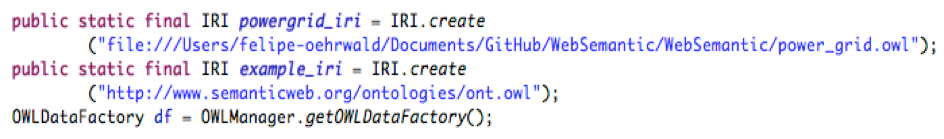
\includegraphics[width=\textwidth]{img/load.png}
\caption{Load an IRI based on the OWL File.}
\label{fig:Load}
\end{figure}

\begin{figure}[h]
\centering
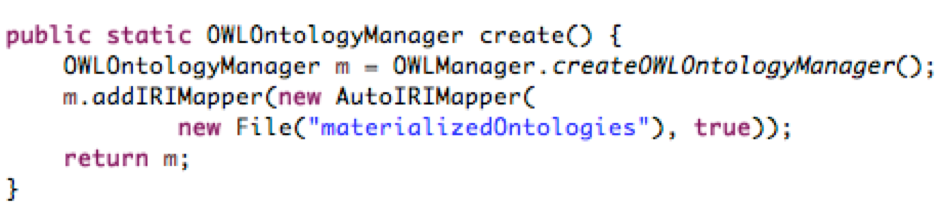
\includegraphics[width=\textwidth]{img/create.png}
\caption{Creates an IRI based on the OWL File.}
\label{fig:Create}
\end{figure}

\newpage

\begin{figure}[h]
\centering
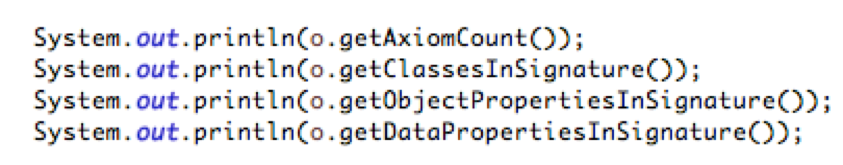
\includegraphics[width=\textwidth]{img/apiCall.png}
\caption{Executing request on OWL Ontology.}
\label{fig:apiCall}
\end{figure}

\begin{figure}[h]
\centering
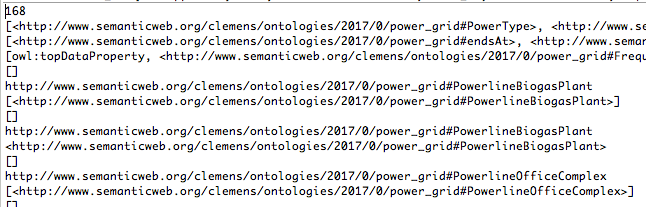
\includegraphics[width=\textwidth]{img/request.png}
\caption{Result of the Java Request.}
\label{fig:request}
\end{figure}

\\
The output reveals that it is possible to run simple request on an OWL Ontology that have been created in Protege. 
With the request we received the size  of the classes that are in the signature of this object (168 in total) or the names of the classes that have been build in the referenced ontology.

\newpage

 

